\documentclass[tikz,border=10pt]{standalone}
\usepackage{tikz}
\begin{document}
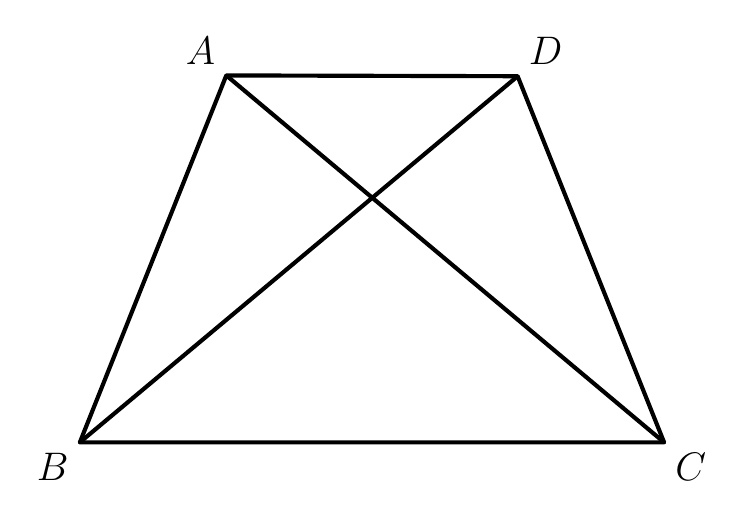
\begin{tikzpicture}[line join=round, line width=1.5pt]
  % Vertices: previous coords scaled by 1.03 about the centre to match original proportions
  \coordinate (A) at (-1.86,2.33);
  \coordinate (B) at (-3.72,-2.33);
  \coordinate (C) at (3.70,-2.33);
  \coordinate (D) at (1.84,2.32);
  % Diagonal intersection: kept as an unlabelled point (no node drawn)
  \coordinate (O) at (0.00,0.77);

  % Sides AB, BC, CD, DA
  \draw (A) -- (B) -- (C) -- (D) -- cycle;

  % Diagonals AC and BD
  \draw (A) -- (C);
  \draw (B) -- (D);

  % Vertex labels (font from STYLE METRICS)
  \node[font=\fontsize{15.5}{18.6}\selectfont, above left] at (A) {$A$};
  \node[font=\fontsize{15.5}{18.6}\selectfont, below left] at (B) {$B$};
  \node[font=\fontsize{15.5}{18.6}\selectfont, below right] at (C) {$C$};
  \node[font=\fontsize{15.5}{18.6}\selectfont, above right] at (D) {$D$};
\end{tikzpicture}
\end{document}